\documentclass[main.tex]{subfiles}

\begin{document}
\section{Introduction}
\subsection{Problem Overview}
\begin{frame}{Wireless Underground Sensor Networks}
	\begin{itemize}
		\item A network consisting of sensor nodes deployed underground.
		\item Sensors collect and send data via wireless connections.
		\item {
			Network lifetime: time from network initialization to shutoff. Shutoff happens when:
			\begin{itemize}
				\item 1 node runs out of energy. (N of N)
				\item N - K + 1 nodes run out of energy. (K of N)
			\end{itemize}
		}
	\end{itemize}

	\begin{center}
    	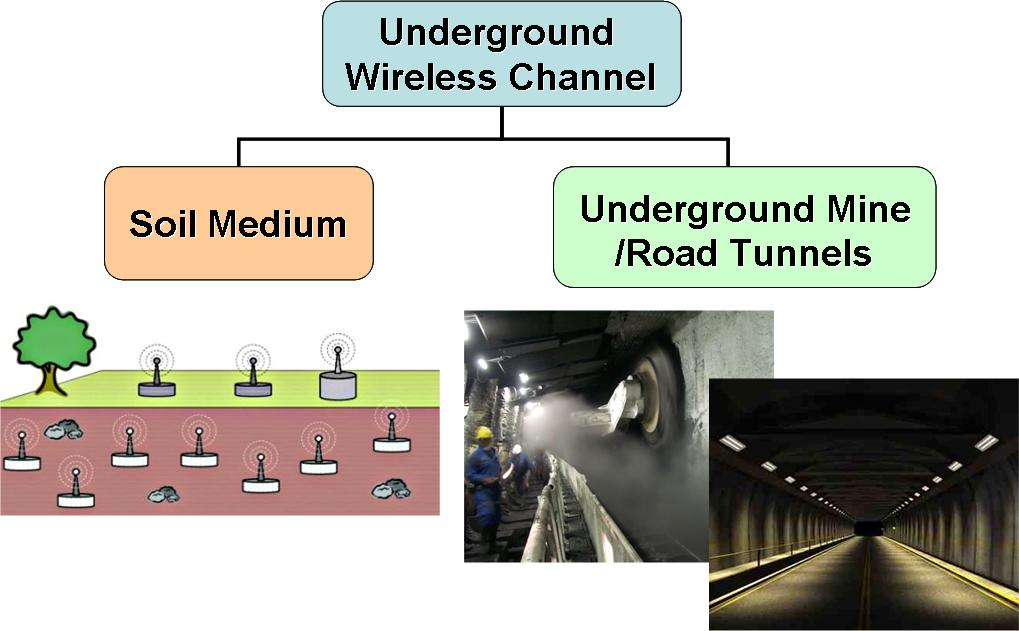
\includegraphics[scale=0.19]{WusnExample.png}
	\end{center}
\end{frame}

\begin{frame}{Applications}
	\begin{itemize}
		\item Agriculture
		\item Infrastructure monitoring
		\item Locating targets
		\item ...
	\end{itemize}
\end{frame}

\begin{frame}{Challenges}{Networking}
	\begin{itemize}
		\item Many models only consider homogenous networks. \footnote{C. Bettstetter, \textit{On the Minimum Node Degree and Connectivity of a Wireless Multihop Network}, ACM MOBIHOC, Lausanne, Switzerland, (2002)} \footnote{Z. Kong and M. Y. Edmund, \textit{Connectivity and Latency in Large Scale Wireless Networks with Unreliable Links}, IEEE INFOCOM ’08, Phoenix, USA, (2008)}
		\item Simple models for above ground networks are insufficient for 2-level networks.
	\end{itemize}
\end{frame}

\begin{frame}{Challenges}{Networking}
	\begin{itemize}
		\item In \footnote{F. Fabbri and R. Verdone, \textit{A Statistical Model for the Connectivity of Nodes in a Multi-Sink Wireless Sensor Network Over a Bounded Region}, European Wireless Conference, Czech Republic, (2008)}, underground sensors are considered. However sensors are assumed to connect to sinks via a sigle hop. Only AG channels are considered and mobile sinks are not included.
		\item In \footnote{Zhi Sun, Ian F.Akyildiz, Gerhard P. Hancke, \textit{Dynamic Connectivity in Wireless Underground Sensor Networks}, IEEE Transactions on Wireless Communications, 10(12)p. 4334-4344, (2011)}, all types of node and channels are considered, however only in 2 dimensions.
	\end{itemize}
\end{frame}

\begin{frame}{Challenges}{Transmission}
	\begin{itemize}
		\item Transmission loss differs in different environments (soil, air).
		\item Transmission loss also affects a node's range. 2-dimensional models are inappropriate.
		\item A node's height/depth needs to be considered in a model.
	\end{itemize}
\end{frame}

\begin{frame}{Challenges}{Energy}
	\begin{itemize}
		\item Key challenge as underground sensors are generally difficult to charge.
		\item { 
			Uses above-ground relay nodes to alleviate network traffic.
			\begin{itemize}
				\item Relay positions are affected by terrain.
				\item Signal loss due to multi environment transmission.
				\item Relays themselves need to be load-balanced for optimal lifetime.
			\end{itemize}
		}
	\end{itemize}
\end{frame}

\begin{frame}{Relay Placement}
	\begin{itemize}
		\item A network node may be a sensor (SN), relay (RN) or base station (BS).
		\item 2-level network: SNs transmit data to RNs via 1 hop. Transmission channels: UG-UG, UG-AG, AG-AG.
		\pause
		\item {
			Goal: Given a network of deployed sensors, maximize the network's lifetime by placing relay nodes.
			\pause
			\begin{itemize}
				\item The number of placed relay must equal $Y$.
				\item Each sensor may only be assigned to 1 relay.
				\item Each relay may only handle $N/Y$ sensors.
			\end{itemize}
		}
	\end{itemize}
\end{frame}

\subsection{Modeling}
\begin{frame}{Transmission Model}
	\begin{columns}[T]
	\begin{column}{.48\textwidth}
		\begin{center}
			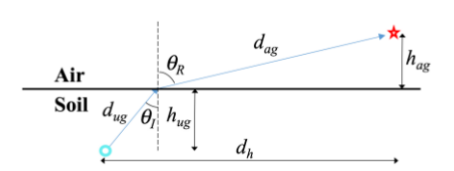
\includegraphics[scale=0.4]{transmission.png}
		\end{center}
	\end{column}	
	\hfill
	\begin{column}{.48\textwidth}
		\begin{itemize}
		 \item $T_{UG-AG} = T_{UG} + T_{AG} + T_R$
		 \item $T_{AG} = -147.6 + 10\eta\log(d_{ag}) + 20\log(f)$
		 \item $T_{UG} = 6.4 + 20\log(d_{ug}) + 20\log\beta + 8.69\alpha d_{ug}$
		 \item $T_R = 0$
		\end{itemize}
	\end{column}	
	\end{columns}
\end{frame}

\begin{frame}{Problem Model (1)}
	\begin{itemize}
		\item {
			Input:
			\begin{itemize}
				\item $S = \{s_1, s_2, ..., s_N \}$: set containing all sensor nodes (SN).
				\item $F = \{f_1, f_2, ..., f_M \}$: set containing all possible relay positions (RN).
				\item $Y$: required number of relays to deploy.
				\item $T = (t_{nm})_{NxM}$: transmission loss for each SN-RN pair. Calculated using the transmission model.
			\end{itemize}					
		}
		
		\item {
			Output:
			\begin{itemize}
				\item $A = (a_{nm})_{NxM}$: decision variable where $a_{nm} = 1$ iff $s_n$ is assigned to $f_m$.
			\end{itemize}					
		}
		
		\item {
			Constraints:
			\begin{itemize}
				\item $\sum_{m=1}^{M} a_{nm} = 1\ \forall n = 1,...,N$
				\item $|\{ m | \sum_{n=1}^N a_{nm} > 0, m = 1,...,M \}| = Y$
				\item $\sum_{n=1}^N a_{nm} \in \{ 0, N/Y \}, m = 1,...,M$. This assumes $Y$ is always divisible by $N$.
			\end{itemize}					
		}
	\end{itemize}
\end{frame}

\begin{frame}{Problem Model (2)}
\begin{itemize}
	\item We can simplify constraints by adding another variable $Z = (z_m)_{1xM}$, $z_m = 1$ iff a relay is deployed at $f_m$.
	\item {
		Rewrite constraints:
		\begin{itemize}
			\item $\sum_{m=1}^M z_m = Y$
			\item $\sum_{n=1}^N a_{nm} . z_m = N/Y, m = 1,...,M$
			\item $\sum_{m=1}^M a_{nm} . z_m = 1, n = 1,...,N$  
		\end{itemize}
	}
	\item {
		We can also formulate the loss function:
		\begin{itemize}
			\item $T_c = max_{n=1}^N (\sum_{m=1}^M t_{nm} . a_{nm} . z_{m})$ (N of N)
			\item $T_c = {max_{N-K+1}}_{n=1}^N (\sum_{m=1}^M t_{nm} . a_{nm} . z_{m})$ (K of N)
		\end{itemize}
	}
	\item The problem can be reduced to Boolean LP and is therefore NP-complete.
\end{itemize}
\end{frame}
\end{document}
